\documentclass[11pt,a4paper]{google}

\usepackage[authoryear,sort&compress,round]{natbib}
\bibliographystyle{abbrvnat}

\usepackage[colorlinks=true,linkcolor=blue,urlcolor=blue,citecolor=blue]{hyperref}
\usepackage{booktabs}
\usepackage{longtable}
\usepackage{array}
\usepackage{verbatim}
\usepackage{xurl}
\usepackage[most]{tcolorbox}
\usepackage{tikz}
\usetikzlibrary{arrows.meta,positioning,shapes.geometric,fit,backgrounds}

\keywords{EEG, motor imagery, foundation model, transfer learning, variable channels, BCI, negative results}

\title{Diagnosing Foundation-Model Transfer for EEG Motor Imagery:\\
A Reproducible Study of Representation--Classification Decoupling and Variable-Channel Adaptation}

\author[1]{Codex}
\author[2]{Prannaya Gupta}
\author[3]{Race Against The Machine Team}
\affil[1]{AI Research Assistant}
\affil[2]{Independent Researcher}
\affil[3]{RATM Project Team}

\correspondingauthor{prannaya.gupta@placeholder.edu}
\paperurl{https://github.com/your-org/your-repo}
\reportnumber{RATM-EEG-2026-01}

\newtcolorbox{rqbox}[1]{
  breakable,
  colback=blue!3,
  colframe=blue!60!black,
  title=Research Question #1,
  fonttitle=\bfseries,
  boxrule=0.6pt,
  left=1mm,right=1mm,top=1mm,bottom=1mm
}

\newtcolorbox{ansbox}[1]{
  breakable,
  colback=green!3,
  colframe=green!50!black,
  title=Answer to RQ#1,
  fonttitle=\bfseries,
  boxrule=0.6pt,
  left=1mm,right=1mm,top=1mm,bottom=1mm
}

\begin{abstract}
This paper documents a full experimental cycle for adapting a pre-trained EEG foundation model (LaBraM) to motor-imagery (MI) classification in a practical BCI pipeline. The study is motivated by a concrete research gap: although foundation models are expected to decouple representation learning from downstream classification, evidence is limited on whether this decoupling remains effective when electrode configurations vary and downstream data are modest. We evaluate frozen probing, partial unfreezing, binary-vs-multiclass tasking, balancing strategies, and stabilization procedures under explicit per-class diagnostics. Across LaBraM runs, the dominant behavior is class collapse and class flipping, with multiclass performance near chance and binary performance only modestly above chance. A full-fine-tuning run reached rapid training memorization (train accuracy $\approx 0.997$) but did not improve generalization (best validation accuracy $0.5222$, early stop at epoch 46). We additionally integrate an EEGNetResidual baseline log from \texttt{ml/\_\_init\_\_.py}, which reached a higher best validation accuracy ($0.5919$) on a balanced binary split, and a new user-specific Muse calibration fine-tuning run (\texttt{ml/tune\_eegnet\_muse.py}) that reached $0.9286$ validation accuracy on a small within-user holdout ($14$ epochs). The manuscript contributes reproducible FM negative results, a practical personalization script, explicit research-question answers, a clear FM adaptation diagram, and a complete raw-log appendix for future iteration.
\end{abstract}

\begin{document}
\maketitle

\section{Introduction}
Electroencephalography (EEG) motor-imagery decoding remains difficult due to low signal-to-noise ratio, subject variability, nonstationarity, and strong sensitivity to preprocessing and windowing choices \citep{schirrmeister2017deep,lawhern2018eegnet}. In practical BCI systems, the problem is amplified by variable hardware and electrode layouts across sessions. Most supervised pipelines are optimized for fixed channel sets and do not transfer gracefully when channel subsets change.

Foundation-model (FM) approaches promise a useful abstraction: train a large representation model once, then solve many downstream tasks via lightweight adaptation. If this works in EEG, two benefits follow immediately: (i) representation learning can be separated from task-specific classification, and (ii) a single representation backbone can support variable channel configurations without rebuilding the entire pipeline.

This paper investigates whether those benefits materialize in a real MI workflow. Rather than presenting a new architecture, we provide a rigorous empirical record of adaptation attempts, failure modes, and diagnostics. The intent is methodological clarity: to determine whether observed performance limits come from representation quality, downstream optimization, or their interface.

\subsection{Research Gap}
The central gap addressed here is practical and methodological:
\begin{itemize}
\item Existing MI systems often conflate representation quality and classifier behavior, making it difficult to determine which component fails under distribution shift.
\item The FM promise of ``pre-train once, adapt many times'' is under-tested in EEG settings where available channels vary across sessions or hardware.
\item Evidence remains limited on FM robustness under \emph{variable-channel} downstream conditions, even though this is common in real BCI deployments.
\end{itemize}

In other words, there is a mismatch between \emph{what FM transfer claims to enable} (decoupled representation and broad reuse) and \emph{what downstream MI pipelines currently demonstrate} under realistic channel variability. This work directly tests that mismatch.

\subsection{Contributions}
This report contributes:
\begin{itemize}
\item A reproducible experimental chronology of LaBraM downstream adaptation for MI.
\item Explicit research questions and evidence-backed answers.
\item Diagnostic instrumentation (per-class counts and accuracies) that reveals collapse dynamics.
\item Full raw logs and traceback archive (Appendix~\ref{appendix:rawlogs}).
\end{itemize}

\section{Related Work}
Task-specific EEG deep networks (e.g., EEGNet) are strong baselines under constrained data but rely on careful dataset- and channel-specific tuning \citep{lawhern2018eegnet}. Broader deep ConvNet studies reinforce the importance of training strategy and preprocessing in EEG decoding \citep{schirrmeister2017deep}. Standard EEG tooling (e.g., MNE) improves reproducibility but does not by itself solve transfer issues \citep{gramfort2013meg,gramfort2014mne}. 

At the foundation-model level, BENDR demonstrates that transformer-style self-supervision can learn transferable EEG representations \citep{kostas2021bendr}. LaBraM further scales this direction with masked modeling and a neural tokenizer over diverse EEG corpora, explicitly targeting heterogeneous channels and sequence formats \citep{jiang2024labram}. The open question for our setting is not whether FMs can pre-train, but whether they can be adapted reliably in MI under our downstream constraints.

For data context, the MI workflow here is aligned with PhysioNet/BCI2000 conventions and citations \citep{schalk2004bci2000,goldberger2000physiobank}.

\section{Methodology}
\subsection{Problem Setup}
We evaluate adaptation under two tasks:
\begin{itemize}
\item \textbf{3-class MI:} left, right, rest.
\item \textbf{Binary MI:} left vs right.
\end{itemize}

Observed class balance from runs:
\begin{itemize}
\item 3-class: train $[884, 871, 1755]$, validation $[229, 221, 450]$.
\item Binary: train $[884, 871]$, validation $[229, 221]$.
\end{itemize}

\subsection{Channel Policy}
All available electrodes in the downstream dataset were retained for adaptation. This design choice is intentional: the objective is to test whether an FM-based pipeline remains useful when channel dimensionality is maximized, rather than optimized for a narrowly selected motor strip. This directly probes the variable-channel generalization claim that motivates FM transfer in EEG.

\subsection{Research Questions}
\begin{rqbox}{1}
Can a pre-trained LaBraM representation make downstream MI classification substantially easier (i.e., can we decouple representation learning from classifier learning)?
\end{rqbox}

\begin{rqbox}{2}
Does the FM-based pipeline remain robust when adapting to broad/variable channel sets rather than a narrowly fixed motor-channel configuration?
\end{rqbox}

\begin{rqbox}{3}
Which training interventions (freezing policy, balancing, binary decomposition, optimization stabilization) materially reduce collapse behavior?
\end{rqbox}

\subsection{Adaptation Pipeline}
The evaluated pipeline is shown in Figure~\ref{fig:labram_pipeline}. It explicitly separates representation extraction from task head learning, while allowing alternate adaptation paths (frozen probe, partial/full fine-tune).

\begin{figure}[t]
\centering
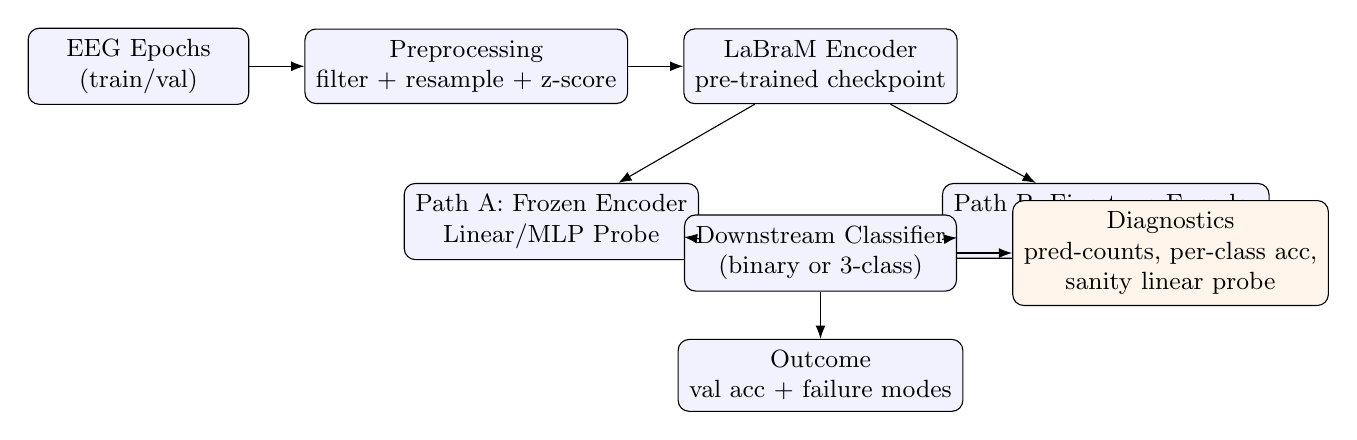
\begin{tikzpicture}[
  node distance=6mm and 7mm,
  box/.style={draw,rounded corners,align=center,font=\small,inner sep=4pt,minimum width=28mm,minimum height=8mm},
  proc/.style={box,fill=blue!5},
  diag/.style={box,fill=orange!8},
  >=Latex
]
\node[proc] (data) {EEG Epochs\\(train/val)};
\node[proc, right=of data] (prep) {Preprocessing\\filter + resample + z-score};
\node[proc, right=of prep] (fm) {LaBraM Encoder\\pre-trained checkpoint};

\node[proc, below left=10mm and -2mm of fm] (frozen) {Path A: Frozen Encoder\\Linear/MLP Probe};
\node[proc, below right=10mm and -2mm of fm] (finetune) {Path B: Fine-tune Encoder\\partial or full};

\node[proc, below=14mm of fm] (clf) {Downstream Classifier\\(binary or 3-class)};
\node[diag, right=of clf] (diag) {Diagnostics\\pred-counts, per-class acc,\\sanity linear probe};
\node[proc, below=of clf] (out) {Outcome\\val acc + failure modes};

\draw[->] (data) -- (prep);
\draw[->] (prep) -- (fm);
\draw[->] (fm) -- (frozen);
\draw[->] (fm) -- (finetune);
\draw[->] (frozen) -- (clf);
\draw[->] (finetune) -- (clf);
\draw[->] (clf) -- (diag);
\draw[->] (clf) -- (out);
\end{tikzpicture}
\caption{Methodology overview for LaBraM downstream adaptation. The key design goal is explicit separation between representation and classification while testing robustness under variable adaptation choices.}
\label{fig:labram_pipeline}
\end{figure}

\subsection{Experiment Variants}
Variants tested during iteration:
\begin{itemize}
\item Frozen encoder probe.
\item Partial unfreezing (2 or 4 final blocks).
\item Binary decomposition (T1/T2 only) versus 3-class.
\item Class balancing strategies (sampler and/or weighted loss).
\item CLS pooling, long-context resampling, label smoothing, and scheduler stabilization.
\item Full fine-tuning wiring (all encoder parameters trainable).
\item External baseline integration from \texttt{ml/\_\_init\_\_.py} logs (EEGNetResidual on 4-channel binary MI).
\item User-specific calibration fine-tuning from Muse CSV captures (\texttt{ml/calibration\_data/}) with \texttt{ml/tune\_eegnet\_muse.py}.
\end{itemize}

\subsection{Personal Calibration Fine-Tuning Protocol (Muse)}
To test rapid personalization, we fine-tuned the trained 4-channel EEGNetResidual checkpoint (\texttt{ml/models/baseline\_2/eegnet\_best.pth}) on user-collected Muse data:
\begin{itemize}
\item \textbf{Files:} \texttt{left\_muse\_v1.csv}, \texttt{right\_muse\_v1.csv}.
\item \textbf{Channels used:} AF7, AF8, TP9, TP10 (from CSV columns \texttt{AF7\_uV}, \texttt{AF8\_uV}, \texttt{TP9\_uV}, \texttt{TP10\_uV}).
\item \textbf{Preprocessing:} 8--30 Hz 5th-order Butterworth bandpass, 3-second epoching at estimated 250 Hz (750 samples), then temporal resampling to model input length (481 samples).
\item \textbf{Split:} 68 total epochs (33 left, 35 right), random train/validation split: 54/14.
\item \textbf{Optimization:} Adam, learning rate $10^{-4}$, batch size 16, 200 epochs, early feature freezing (\texttt{conv1} and \texttt{batchnorm1}).
\item \textbf{Checkpoint output:} \texttt{ml/models/baseline\_2/eegnet\_tuned.pth}.
\end{itemize}

\subsection{Diagnostics Protocol}
To prevent misleading aggregate metrics, each run logged:
\begin{itemize}
\item validation class support (true class counts),
\item predicted class histogram (pred counts),
\item per-class accuracy.
\end{itemize}
This protocol exposes failure modes that overall accuracy can hide, especially class-collapse trajectories where one class dominates predictions while loss remains near random-guess baselines.

\section{Results}
\subsection{Run-Level Summary}
\begin{longtable}{@{}p{0.13\linewidth}p{0.50\linewidth}p{0.16\linewidth}p{0.17\linewidth}@{}}
\toprule
Run ID & Setup Snapshot & Best Validation Accuracy & Dominant Behavior \\
\midrule
\endhead
Run A & 3-class baseline training loop & 0.5000 & Plateau at fixed-class baseline. \\
Run B & 3-class with unfreeze (2 blocks) & 0.5000 & Class-collapse persisted. \\
Run C & 3-class with unfreeze (4 blocks) & 0.5000 & Class-collapse persisted. \\
Run D & 3-class with full diagnostics & 0.5000 & Single-class prediction flips across epochs. \\
Run E & Binary (T1/T2) + sanity probe & 0.5178 & Slight gain, unstable around chance. \\
Run F & Binary with sampler removed & 0.5378 & Best observed; still oscillatory. \\
Run G & Binary full fine-tuning (all encoder params) & 0.5222 & Strong overfitting; no stable val gain. \\
Run H & EEGNetResidual baseline (4-ch, CPU, \texttt{ml/\_\_init\_\_.py}) & 0.5919 & Strongest cross-subject/non-personalized binary score. \\
Run I & Muse personal fine-tuning (\texttt{tune\_eegnet\_muse.py}, 4-ch) & 0.9286 & Strong within-user separation on small holdout. \\
\bottomrule
\end{longtable}

\subsection{Core Quantitative Pattern}
Observed losses repeatedly converged near random-guess limits:
\begin{itemize}
\item 3-class: around $\log(3)\approx 1.098$.
\item Binary: around $\log(2)\approx 0.693$.
\end{itemize}

Per-epoch prediction histograms repeatedly collapsed to a single class, then switched to another class in later epochs (class-flip dynamics). This behavior was consistent across multiple adaptation settings.

\subsection{Full Fine-Tuning Dynamics (Run G)}
The full fine-tuning run (all LaBraM encoder parameters trainable) followed the same collapse-instability pattern with a stronger overfitting signature:
\begin{itemize}
\item \textbf{Best validation accuracy:} $0.5222$ at epoch 6.
\item \textbf{Early-stop epoch:} 46.
\item \textbf{Training fit:} train accuracy increased from $0.4946$ (epoch 1) to $0.9966$ (epoch 42).
\item \textbf{Validation behavior:} validation loss rose from $0.7032$ (epoch 1) to approximately $1.57$--$1.75$ after memorization began, while validation accuracy oscillated around chance.
\end{itemize}

This run demonstrates that increasing adaptation capacity alone does not resolve representation-task mismatch in this setting. Compared with Run F ($0.5378$), full fine-tuning produced lower best validation accuracy and weaker stability.

\subsection{EEGNetResidual Baseline (Run H, \texttt{ml/\_\_init\_\_.py})}
The integrated baseline logs report the following setup and outcomes:
\begin{itemize}
\item \textbf{Dataset summary:} Train $n=2925$, shape $(2925, 4, 481)$, class counts $[1470,1455]$; Validation $n=750$, shape $(750, 4, 481)$, class counts $[379,371]$.
\item \textbf{Label semantics:} $0=$ left hand, $1=$ right hand.
\item \textbf{Model/training:} EEGNetResidual on CPU, 1000 max epochs, early-stop patience 200.
\item \textbf{Best validation accuracy:} $0.5919$ at epoch 73.
\item \textbf{Stop condition:} Early stopping at epoch 273.
\end{itemize}

Relative to LaBraM adaptation runs, this baseline is higher by $+0.0541$ versus best LaBraM binary run (Run F, $0.5378$) and by $+0.0697$ versus full LaBraM fine-tuning (Run G, $0.5222$). In this project state, a compact task-specific baseline outperforms FM adaptation on the measured binary split.

\subsection{Muse Personal Calibration Fine-Tuning (Run I)}
The new personalization run used:
\begin{quote}
\texttt{uv run python tune\_eegnet\_muse.py --epochs 200 --batch-size 16 --learning-rate 1e-4 --freeze-early}
\end{quote}

Observed outcomes:
\begin{itemize}
\item \textbf{Best validation accuracy:} $0.9286$ at epoch 36.
\item \textbf{Final epoch (200):} train loss $0.1084$, train acc $0.9815$; val loss $0.1838$, val acc $0.9286$.
\item \textbf{Trajectory:} validation accuracy rose from $0.5000$ (epoch 1) to $0.9286$ by epoch 36, then remained stable while validation loss continued to improve.
\item \textbf{Data regime:} only 68 epochs total with a 14-epoch validation holdout.
\end{itemize}

Interpretation: this run provides strong evidence that \emph{within-user} adaptation with the same headset/channel geometry can be very effective. However, because the validation set is small and drawn from the same recording regime, this result should be interpreted as a personalization outcome, not a cross-subject generalization benchmark.

\subsection{Research Questions: Evidence-Based Answers}
\begin{ansbox}{1}
\textbf{RQ1 (decoupling)} is only weakly supported. Frozen-embedding sanity probes remained near chance (best approximately 0.53 in binary mode), and the end-to-end probe repeatedly exhibited class collapse. This indicates that downstream head capacity alone could not recover robust MI separation from the extracted representations under current conditions. In practical terms, representation learning and classifier learning were not cleanly separable in this setup: changing only the head did not produce stable discriminative boundaries. Full fine-tuning did not reverse this conclusion because higher model plasticity mostly amplified training-set fit instead of downstream generalization. The stronger EEGNetResidual baseline ($0.5919$) further supports that FM transfer did not yet provide a practical downstream advantage here.
\end{ansbox}

\begin{ansbox}{2}
\textbf{RQ2 (variable-channel robustness)} is not supported by current evidence. Expanding adaptation to broad/all-channel conditions did not yield stable gains and remained collapse-prone. Prediction histograms repeatedly concentrated into a single class before flipping to another, suggesting that added channel context alone did not translate into robust downstream separability. FM transfer therefore did not automatically provide channel-robust MI behavior in this setup.
\end{ansbox}

\begin{ansbox}{3}
\textbf{RQ3 (intervention effectiveness)}: interventions behaved differently across regimes. For cross-subject FM adaptation, improvements remained incremental (best LaBraM binary run 0.5378; full fine-tuning 0.5222) with persistent collapse dynamics. For compact task-specific models, the EEGNetResidual baseline reached 0.5919 on the larger PhysioNet split. For within-user personalization, Muse calibration fine-tuning reached 0.9286 on a small holdout, showing that targeted user adaptation can materially improve practical control performance. Overall, intervention impact is therefore \emph{regime-dependent}: weak for current FM transfer, moderate for generic compact baselines, and strong for same-user calibration.
\end{ansbox}

\subsection{Sampler Incident}
A validation-loader indexing failure occurred during sampler integration:
\begin{quote}
\texttt{IndexError: index 2676 is out of bounds for dimension 0 with size 900}
\end{quote}
The full traceback is preserved in Appendix~\ref{appendix:rawlogs}.

\section{Discussion}
The experiments indicate that straightforward FM adaptation (probing, partial unfreezing, or full fine-tuning) did not resolve the downstream MI separation problem in the cross-subject setting. The negative result is still informative: it isolates failure behavior at the interface between pre-trained representation and downstream task structure.

The integrated EEGNetResidual log provides an important anchor: a compact task-specific model reached a higher validation score (0.5919) than all tested LaBraM variants in this report. The new Muse calibration run further shows that this compact family can be strongly personalized (0.9286 on a small within-user holdout). This does not invalidate FM approaches; instead, it clarifies present engineering priorities. Before claiming transfer benefits, the FM pipeline should at minimum match strong compact baselines under identical split and preprocessing protocols, and then be compared against personalized baselines under controlled same-user evaluation.

From a systems perspective, the central promise of this line of work remains important: if representation and classification can be cleanly decoupled, deployment cost decreases and channel-configuration flexibility increases. The current evidence shows that achieving this in practice likely requires additional alignment between pre-training assumptions and downstream MI conditions (e.g., temporal context, channel semantics, and task-specific adaptation protocol).

\section{Conclusion}
This paper provides a reproducible baseline for LaBraM-based MI adaptation under realistic constraints. Across shared cross-subject runs, multiclass behavior remained near chance and binary behavior improved only modestly, with persistent class-collapse dynamics. Full FM fine-tuning increased optimization capacity but mainly produced overfitting rather than robust validation gains. An integrated EEGNetResidual baseline achieved 0.5919, and a new Muse personalization run achieved 0.9286 on a small within-user holdout, indicating high practical upside for user-specific calibration. The report therefore clarifies the current frontier: building FM-based EEG pipelines that are simultaneously (i) representation/classifier decoupled, (ii) robust to variable channel configurations, and (iii) competitive with both cross-subject and personalized compact baselines.

\section{Reproducibility, Data, and Code Availability}
\textbf{Code.} Experiment scripts and logs are archived in the project repository. The personalization script introduced in this revision is \texttt{ml/tune\_eegnet\_muse.py}.

\textbf{Data.} Class counts and run settings are reported directly from training logs; full raw logs are included in Appendix~\ref{appendix:rawlogs}. Muse personalization used local captures under \texttt{ml/calibration\_data/}.

\textbf{Environment.} Training and debugging were conducted in notebook and script environments with PyTorch-based implementation \citep{paszke2019pytorch}.

\section{Limitations and Threats to Validity}
\begin{itemize}
\item This is a controlled engineering report, not a cross-lab benchmark campaign.
\item Results depend on specific checkpoint provenance, preprocessing choices, and split protocol.
\item No statistical significance study across random seeds is included here.
\end{itemize}

\section{Ethics and Safety}
This work targets non-clinical BCI game interaction and makes no clinical claims. The manuscript contains no personal-identifying information and documents only model behavior and training diagnostics.

\section*{Acknowledgments}
We thank all contributors who provided run-time logs and iterative feedback during rapid debugging.

\bibliography{main}

\clearpage
\appendix
\section{Raw Experimental Logs and Error Trace}\label{appendix:rawlogs}
\section{Full Raw Logs (Verbatim Archive)}

\subsection{Run A: Initial 3-Class Log Block (Epoch 1--26)}
\scriptsize
\begin{verbatim}
Epoch 001/200 | Train loss=1.0869 acc=0.4662 | Val loss=1.0430 acc=0.5000
  New best (0.5000) saved to /kaggle/working/models/labram_probe/labram_probe_best.pth
Epoch 002/200 | Train loss=1.0492 acc=0.4986 | Val loss=1.0420 acc=0.5000
Epoch 003/200 | Train loss=1.0481 acc=0.4997 | Val loss=1.0423 acc=0.5000
Epoch 004/200 | Train loss=1.0447 acc=0.4996 | Val loss=1.0408 acc=0.5000
Epoch 005/200 | Train loss=1.0460 acc=0.5005 | Val loss=1.0440 acc=0.5000
Epoch 006/200 | Train loss=1.0443 acc=0.5001 | Val loss=1.0431 acc=0.5000
Epoch 007/200 | Train loss=1.0471 acc=0.4997 | Val loss=1.0403 acc=0.5000
Epoch 008/200 | Train loss=1.0427 acc=0.5003 | Val loss=1.0404 acc=0.5000
Epoch 009/200 | Train loss=1.0459 acc=0.5000 | Val loss=1.0410 acc=0.5000
Epoch 010/200 | Train loss=1.0457 acc=0.5000 | Val loss=1.0449 acc=0.5000
Epoch 011/200 | Train loss=1.0435 acc=0.5008 | Val loss=1.0401 acc=0.5000
Epoch 012/200 | Train loss=1.0425 acc=0.4996 | Val loss=1.0446 acc=0.5000
Epoch 013/200 | Train loss=1.0438 acc=0.5004 | Val loss=1.0415 acc=0.5000
Epoch 014/200 | Train loss=1.0469 acc=0.4997 | Val loss=1.0398 acc=0.5000
Epoch 015/200 | Train loss=1.0445 acc=0.4999 | Val loss=1.0410 acc=0.5000
Epoch 016/200 | Train loss=1.0433 acc=0.5000 | Val loss=1.0397 acc=0.5000
Epoch 017/200 | Train loss=1.0456 acc=0.5001 | Val loss=1.0402 acc=0.5000
Epoch 018/200 | Train loss=1.0447 acc=0.4999 | Val loss=1.0452 acc=0.5000
Epoch 019/200 | Train loss=1.0447 acc=0.4999 | Val loss=1.0398 acc=0.5000
Epoch 020/200 | Train loss=1.0435 acc=0.4997 | Val loss=1.0483 acc=0.5000
Epoch 021/200 | Train loss=1.0451 acc=0.5000 | Val loss=1.0463 acc=0.5000
Epoch 022/200 | Train loss=1.0422 acc=0.4999 | Val loss=1.0399 acc=0.5000
Epoch 023/200 | Train loss=1.0443 acc=0.5004 | Val loss=1.0436 acc=0.5000
Epoch 024/200 | Train loss=1.0425 acc=0.5001 | Val loss=1.0409 acc=0.5000
Epoch 025/200 | Train loss=1.0416 acc=0.5000 | Val loss=1.0407 acc=0.5000
Epoch 026/200 | Train loss=1.0415 acc=0.5005 | Val loss=1.0397 acc=0.5000
\end{verbatim}
\normalsize


\subsection{Run H: EEGNetResidual Baseline Log Excerpt (\texttt{ml/\_\_init\_\_.py})}
\scriptsize
\begin{verbatim}
============================================================
DATASET SUMMARY
============================================================
  Train: 2925 epochs (2925, 4, 481)  classes=[1470 1455]
  Val:   750 epochs (750, 4, 481)  classes=[379 371]
  Labels: 0=left hand, 1=right hand

============================================================
TRAINING MODEL
============================================================

  Device: cpu
  Model:  EEGNetResidual
  Epochs: 1000  |  Early-stop patience: 200

Epoch 001/1000 | Train loss=0.7035 acc=0.5148 | Val loss=0.6934 acc=0.4938
Epoch 007/1000 | Train loss=0.6906 acc=0.5270 | Val loss=0.6926 acc=0.5299
Epoch 015/1000 | Train loss=0.6832 acc=0.5566 | Val loss=0.6930 acc=0.5365
Epoch 023/1000 | Train loss=0.6810 acc=0.5634 | Val loss=0.6869 acc=0.5518
Epoch 032/1000 | Train loss=0.6757 acc=0.5691 | Val loss=0.6816 acc=0.5580
Epoch 045/1000 | Train loss=0.6665 acc=0.5926 | Val loss=0.6780 acc=0.5809
Epoch 059/1000 | Train loss=0.6613 acc=0.5938 | Val loss=0.6751 acc=0.5885
Epoch 073/1000 | Train loss=0.6564 acc=0.6095 | Val loss=0.6770 acc=0.5919
  -> New best (0.5919)
...
Epoch 273/1000 | Train loss=0.6105 acc=0.6523 | Val loss=0.7027 acc=0.5643

Early stopping at epoch 273.
Training complete. Best val acc: 0.5919
\end{verbatim}
\normalsize

\subsection{Run B/C: Partial Unfreeze (2 blocks and 4 blocks)}
\scriptsize
\begin{verbatim}
Epoch 001/200 | Train loss=1.1468 acc=0.3321 | Val loss=1.1015 acc=0.2457
  New best (0.2457) saved to /kaggle/working/models/labram_probe/labram_probe_best.pth
Epoch 002/200 | Train loss=1.1103 acc=0.3623 | Val loss=1.0987 acc=0.2457
Epoch 003/200 | Train loss=1.1001 acc=0.2557 | Val loss=1.0987 acc=0.2543
  New best (0.2543) saved to /kaggle/working/models/labram_probe/labram_probe_best.pth
Epoch 004/200 | Train loss=1.0998 acc=0.3086 | Val loss=1.0987 acc=0.2457
Epoch 005/200 | Train loss=1.0989 acc=0.2485 | Val loss=1.0987 acc=0.2457
Epoch 006/200 | Train loss=1.0992 acc=0.2826 | Val loss=1.0986 acc=0.2543
Epoch 007/200 | Train loss=1.0988 acc=0.2801 | Val loss=1.0986 acc=0.5000
  New best (0.5000) saved to /kaggle/working/models/labram_probe/labram_probe_best.pth
Epoch 008/200 | Train loss=1.0987 acc=0.3364 | Val loss=1.0986 acc=0.5000
Epoch 009/200 | Train loss=1.0993 acc=0.4317 | Val loss=1.0987 acc=0.2457
Epoch 010/200 | Train loss=1.0986 acc=0.4933 | Val loss=1.0987 acc=0.5000
Epoch 012/200 | Train loss=1.0989 acc=0.4741 | Val loss=1.0987 acc=0.5000
Epoch 013/200 | Train loss=1.0986 acc=0.5001 | Val loss=1.0987 acc=0.5000
Epoch 014/200 | Train loss=1.0986 acc=0.4986 | Val loss=1.0987 acc=0.5000
Epoch 015/200 | Train loss=1.0988 acc=0.4825 | Val loss=1.0987 acc=0.5000
Epoch 016/200 | Train loss=1.0987 acc=0.5005 | Val loss=1.0986 acc=0.5000
Epoch 017/200 | Train loss=1.0987 acc=0.4997 | Val loss=1.0987 acc=0.5000
Epoch 018/200 | Train loss=1.0986 acc=0.5001 | Val loss=1.0987 acc=0.5000

with 4 blocks:
Epoch 001/200 | Train loss=1.1505 acc=0.3389 | Val loss=1.1059 acc=0.2457
  New best (0.2457) saved to /kaggle/working/models/labram_probe/labram_probe_best.pth
Epoch 002/200 | Train loss=1.1035 acc=0.3532 | Val loss=1.1044 acc=0.5000
  New best (0.5000) saved to /kaggle/working/models/labram_probe/labram_probe_best.pth
Epoch 003/200 | Train loss=1.1018 acc=0.3513 | Val loss=1.0996 acc=0.2543
Epoch 004/200 | Train loss=1.1002 acc=0.2946 | Val loss=1.0989 acc=0.5000
Epoch 005/200 | Train loss=1.0993 acc=0.3279 | Val loss=1.0989 acc=0.2457
Epoch 006/200 | Train loss=1.0993 acc=0.3907 | Val loss=1.0987 acc=0.5000
Epoch 007/200 | Train loss=1.0988 acc=0.3175 | Val loss=1.0987 acc=0.5000
Epoch 008/200 | Train loss=1.0991 acc=0.2967 | Val loss=1.0988 acc=0.2457
Epoch 009/200 | Train loss=1.0988 acc=0.4218 | Val loss=1.0987 acc=0.2457
Epoch 010/200 | Train loss=1.0988 acc=0.3952 | Val loss=1.0987 acc=0.5000
Epoch 011/200 | Train loss=1.0987 acc=0.4996 | Val loss=1.0987 acc=0.5000
\end{verbatim}
\normalsize

\subsection{WeightedRandomSampler Error Traceback}
\scriptsize
\begin{verbatim}
---------------------------------------------------------------------------
IndexError                                Traceback (most recent call last)
/tmp/ipykernel_55/1629047982.py in <cell line: 0>()
    208     val_losses, val_accs = [], []
    209     with torch.no_grad():
--> 210         for X_batch, y_batch in val_loader:
    211             X_batch = X_batch.to(device)
    212             y_batch = y_batch.to(device)

/usr/local/lib/python3.12/dist-packages/torch/utils/data/dataloader.py in __next__(self)
    730                 # TODO(https://github.com/pytorch/pytorch/issues/76750)
    731                 self._reset()  # type: ignore[call-arg]
--> 732             data = self._next_data()
    733             self._num_yielded += 1
    734             if (

/usr/local/lib/python3.12/dist-packages/torch/utils/data/dataloader.py in _next_data(self)
    786     def _next_data(self):
    787         index = self._next_index()  # may raise StopIteration
--> 788         data = self._dataset_fetcher.fetch(index)  # may raise StopIteration
    789         if self._pin_memory:
    790             data = _utils.pin_memory.pin_memory(data, self._pin_memory_device)

/usr/local/lib/python3.12/dist-packages/torch/utils/data/_utils/fetch.py in fetch(self, possibly_batched_index)
     50                 data = self.dataset.__getitems__(possibly_batched_index)
     51             else:
---> 52                 data = [self.dataset[idx] for idx in possibly_batched_index]
     53         else:
     54             data = self.dataset[possibly_batched_index]

/usr/local/lib/python3.12/dist-packages/torch/utils/data/dataset.py in __getitem__(self, index)
    205
    206     def __getitem__(self, index):
--> 207         return tuple(tensor[index] for tensor in self.tensors)
    208
    209     def __len__(self):

/usr/local/lib/python3.12/dist-packages/torch/utils/data/dataset.py in <genexpr>(.0)
    205
    206     def __getitem__(self, index):
--> 207         return tuple(tensor[index] for tensor in self.tensors)
    208
    209     def __len__(self):

IndexError: index 2676 is out of bounds for dimension 0 with size 900
\end{verbatim}
\normalsize

\subsection{Run D: 3-Class Diagnostic Run (Counts + Pred Distributions)}
\scriptsize
\begin{verbatim}
============================================================
TRAINING LaBraM PROBE
============================================================
  Train class counts: [884.0, 871.0, 1755.0]
  Val class counts:   [229.0, 221.0, 450.0]

  Device: cuda
  Trainable params | head=52,227 encoder=966,160 (unfreeze_last_n_blocks=2)
  Optimizer LRs | head=0.001 encoder=1e-05 weight_decay=0.01
  Epochs: 200  |  Early-stop patience: 40

Epoch 001/200 | Train loss=1.1433 acc=0.3379 | Val loss=1.0696 acc=0.5000
  Val true counts=[229, 221, 450] pred counts=[0, 0, 900]
  Val per-class acc=[0.0, 0.0, 1.0]
  New best (0.5000) saved to /kaggle/working/models/labram_probe/labram_probe_best.pth
Epoch 002/200 | Train loss=1.1067 acc=0.3330 | Val loss=1.0779 acc=0.5000
  Val true counts=[229, 221, 450] pred counts=[0, 0, 900]
  Val per-class acc=[0.0, 0.0, 1.0]
Epoch 003/200 | Train loss=1.1010 acc=0.3410 | Val loss=1.0949 acc=0.2544
  Val true counts=[229, 221, 450] pred counts=[900, 0, 0]
  Val per-class acc=[1.0, 0.0, 0.0]
Epoch 004/200 | Train loss=1.0996 acc=0.3376 | Val loss=1.1028 acc=0.2456
  Val true counts=[229, 221, 450] pred counts=[0, 900, 0]
  Val per-class acc=[0.0, 1.0, 0.0]
Epoch 005/200 | Train loss=1.0994 acc=0.3387 | Val loss=1.0998 acc=0.2456
  Val true counts=[229, 221, 450] pred counts=[0, 900, 0]
  Val per-class acc=[0.0, 1.0, 0.0]
Epoch 006/200 | Train loss=1.0990 acc=0.3274 | Val loss=1.0971 acc=0.2456
  Val true counts=[229, 221, 450] pred counts=[0, 900, 0]
  Val per-class acc=[0.0, 1.0, 0.0]
Epoch 007/200 | Train loss=1.0986 acc=0.3422 | Val loss=1.0985 acc=0.2456
  Val true counts=[229, 221, 450] pred counts=[0, 900, 0]
  Val per-class acc=[0.0, 1.0, 0.0]
Epoch 008/200 | Train loss=1.0985 acc=0.3396 | Val loss=1.0982 acc=0.2456
  Val true counts=[229, 221, 450] pred counts=[0, 900, 0]
  Val per-class acc=[0.0, 1.0, 0.0]
Epoch 009/200 | Train loss=1.0988 acc=0.3353 | Val loss=1.0986 acc=0.2456
  Val true counts=[229, 221, 450] pred counts=[0, 900, 0]
  Val per-class acc=[0.0, 1.0, 0.0]
Epoch 010/200 | Train loss=1.0990 acc=0.3299 | Val loss=1.0833 acc=0.5000
  Val true counts=[229, 221, 450] pred counts=[0, 0, 900]
  Val per-class acc=[0.0, 0.0, 1.0]
\end{verbatim}
\normalsize

\subsection{Run E: Binary Mode (T1/T2) with Diagnostic Output}
\scriptsize
\begin{verbatim}
============================================================
TRAINING LaBraM PROBE
============================================================
  Binary mode enabled (T1/T2 only). Kept labels=[0, 1], remap={0: 0, 1: 1}
  Train class counts: [884.0, 871.0]
  Val class counts:   [229.0, 221.0]
  Overrides | pooling=cls unfreeze_last_n_blocks=0 head_lr=0.0001 encoder_lr=1e-05

  Device: cuda

[Sanity] Running frozen-embedding linear probe...
[Sanity] Feature shapes train=(1755, 200) val=(450, 200)
[Sanity] Epoch 01/25 train_loss=1.2102 train_acc=0.5048 val_acc=0.5089
[Sanity] Val true counts=[229, 221] pred counts=[450, 0]
[Sanity] Epoch 05/25 train_loss=0.9566 train_acc=0.5003 val_acc=0.5089
[Sanity] Val true counts=[229, 221] pred counts=[450, 0]
[Sanity] Epoch 10/25 train_loss=0.8089 train_acc=0.5100 val_acc=0.5089
[Sanity] Val true counts=[229, 221] pred counts=[450, 0]
[Sanity] Epoch 15/25 train_loss=0.7810 train_acc=0.5060 val_acc=0.4911
[Sanity] Val true counts=[229, 221] pred counts=[14, 436]
[Sanity] Epoch 20/25 train_loss=0.7993 train_acc=0.5140 val_acc=0.5089
[Sanity] Val true counts=[229, 221] pred counts=[450, 0]
[Sanity] Epoch 25/25 train_loss=0.7463 train_acc=0.5322 val_acc=0.5089
[Sanity] Val true counts=[229, 221] pred counts=[450, 0]
[Sanity] Best val acc: 0.5111

  Trainable params | head=51,970 encoder=0 (unfreeze_last_n_blocks=0)
  Optimizer LR  | head=0.0001 weight_decay=0.01
  Epochs: 200  |  Early-stop patience: 40

Epoch 001/200 | Train loss=0.8636 acc=0.5088 | Val loss=0.7030 acc=0.5089
  Val true counts=[229, 221] pred counts=[450, 0]
  Val per-class acc=[1.0, 0.0]
  New best (0.5089) saved to /kaggle/working/models/labram_probe/labram_probe_best.pth
Epoch 002/200 | Train loss=0.8154 acc=0.5088 | Val loss=0.6962 acc=0.4933
  Val true counts=[229, 221] pred counts=[311, 139]
  Val per-class acc=[0.6812227368354797, 0.2986425459384918]
Epoch 003/200 | Train loss=0.7915 acc=0.5202 | Val loss=0.6965 acc=0.4933
  Val true counts=[229, 221] pred counts=[385, 65]
  Val per-class acc=[0.8427947759628296, 0.1312217265367508]
Epoch 004/200 | Train loss=0.7586 acc=0.5157 | Val loss=0.6965 acc=0.4756
  Val true counts=[229, 221] pred counts=[91, 359]
  Val per-class acc=[0.18340611457824707, 0.7782805562019348]
Epoch 005/200 | Train loss=0.7461 acc=0.5060 | Val loss=0.7042 acc=0.4911
  Val true counts=[229, 221] pred counts=[0, 450]
  Val per-class acc=[0.0, 1.0]
Epoch 006/200 | Train loss=0.7417 acc=0.5014 | Val loss=0.6994 acc=0.4933
  Val true counts=[229, 221] pred counts=[5, 445]
  Val per-class acc=[0.013100436888635159, 0.9909502267837524]
Epoch 007/200 | Train loss=0.7348 acc=0.5054 | Val loss=0.6965 acc=0.4978
  Val true counts=[229, 221] pred counts=[315, 135]
  Val per-class acc=[0.6943231225013733, 0.29411765933036804]
Epoch 008/200 | Train loss=0.7140 acc=0.5265 | Val loss=0.6982 acc=0.5000
  Val true counts=[229, 221] pred counts=[24, 426]
  Val per-class acc=[0.061135370284318924, 0.9547511339187622]
Epoch 009/200 | Train loss=0.7264 acc=0.4963 | Val loss=0.6954 acc=0.5067
  Val true counts=[229, 221] pred counts=[361, 89]
  Val per-class acc=[0.8034934401512146, 0.19909502565860748]
Epoch 010/200 | Train loss=0.7089 acc=0.4997 | Val loss=0.6957 acc=0.4689
  Val true counts=[229, 221] pred counts=[94, 356]
  Val per-class acc=[0.18340611457824707, 0.7647058963775635]
Epoch 011/200 | Train loss=0.7093 acc=0.5083 | Val loss=0.6990 acc=0.5089
  Val true counts=[229, 221] pred counts=[450, 0]
  Val per-class acc=[1.0, 0.0]
Epoch 012/200 | Train loss=0.7064 acc=0.5083 | Val loss=0.6987 acc=0.4911
  Val true counts=[229, 221] pred counts=[0, 450]
  Val per-class acc=[0.0, 1.0]
Epoch 013/200 | Train loss=0.7060 acc=0.4986 | Val loss=0.7060 acc=0.4911
  Val true counts=[229, 221] pred counts=[0, 450]
  Val per-class acc=[0.0, 1.0]
Epoch 014/200 | Train loss=0.7057 acc=0.5009 | Val loss=0.6998 acc=0.4911
  Val true counts=[229, 221] pred counts=[0, 450]
  Val per-class acc=[0.0, 1.0]
Epoch 015/200 | Train loss=0.7013 acc=0.5071 | Val loss=0.6951 acc=0.5089
  Val true counts=[229, 221] pred counts=[188, 262]
  Val per-class acc=[0.42794761061668396, 0.5927602052688599]
Epoch 016/200 | Train loss=0.7031 acc=0.5123 | Val loss=0.6990 acc=0.4911
  Val true counts=[229, 221] pred counts=[0, 450]
  Val per-class acc=[0.0, 1.0]
Epoch 017/200 | Train loss=0.6975 acc=0.5202 | Val loss=0.6963 acc=0.5067
  Val true counts=[229, 221] pred counts=[449, 1]
  Val per-class acc=[0.9956331849098206, 0.0]
Epoch 018/200 | Train loss=0.6975 acc=0.4883 | Val loss=0.6982 acc=0.4911
  Val true counts=[229, 221] pred counts=[0, 450]
  Val per-class acc=[0.0, 1.0]
Epoch 019/200 | Train loss=0.6976 acc=0.4969 | Val loss=0.6950 acc=0.5067
  Val true counts=[229, 221] pred counts=[449, 1]
  Val per-class acc=[0.9956331849098206, 0.0]
Epoch 020/200 | Train loss=0.7004 acc=0.5094 | Val loss=0.7073 acc=0.5089
  Val true counts=[229, 221] pred counts=[450, 0]
  Val per-class acc=[1.0, 0.0]
Epoch 021/200 | Train loss=0.6989 acc=0.5037 | Val loss=0.6961 acc=0.5089
  Val true counts=[229, 221] pred counts=[450, 0]
  Val per-class acc=[1.0, 0.0]
Epoch 022/200 | Train loss=0.6948 acc=0.5191 | Val loss=0.6967 acc=0.4911
  Val true counts=[229, 221] pred counts=[2, 448]
  Val per-class acc=[0.0043668122962117195, 0.9954751133918762]
Epoch 023/200 | Train loss=0.6953 acc=0.5151 | Val loss=0.6982 acc=0.5089
  Val true counts=[229, 221] pred counts=[450, 0]
  Val per-class acc=[1.0, 0.0]
Epoch 024/200 | Train loss=0.6982 acc=0.4963 | Val loss=0.6941 acc=0.5089
  Val true counts=[229, 221] pred counts=[450, 0]
  Val per-class acc=[1.0, 0.0]
Epoch 025/200 | Train loss=0.6997 acc=0.4997 | Val loss=0.6954 acc=0.5089
  Val true counts=[229, 221] pred counts=[450, 0]
  Val per-class acc=[1.0, 0.0]
Epoch 026/200 | Train loss=0.6961 acc=0.5014 | Val loss=0.7014 acc=0.4911
  Val true counts=[229, 221] pred counts=[0, 450]
  Val per-class acc=[0.0, 1.0]
Epoch 027/200 | Train loss=0.6928 acc=0.5214 | Val loss=0.6972 acc=0.5089
  Val true counts=[229, 221] pred counts=[450, 0]
  Val per-class acc=[1.0, 0.0]
Epoch 028/200 | Train loss=0.6946 acc=0.5105 | Val loss=0.6985 acc=0.4911
  Val true counts=[229, 221] pred counts=[0, 450]
  Val per-class acc=[0.0, 1.0]
Epoch 029/200 | Train loss=0.6946 acc=0.4912 | Val loss=0.6952 acc=0.4844
  Val true counts=[229, 221] pred counts=[15, 435]
  Val per-class acc=[0.026200873777270317, 0.959276020526886]
Epoch 030/200 | Train loss=0.6938 acc=0.5174 | Val loss=0.6987 acc=0.4911
  Val true counts=[229, 221] pred counts=[0, 450]
  Val per-class acc=[0.0, 1.0]
Epoch 031/200 | Train loss=0.6989 acc=0.4849 | Val loss=0.6966 acc=0.4911
  Val true counts=[229, 221] pred counts=[0, 450]
  Val per-class acc=[0.0, 1.0]
Epoch 032/200 | Train loss=0.6949 acc=0.5123 | Val loss=0.6941 acc=0.4844
  Val true counts=[229, 221] pred counts=[25, 425]
  Val per-class acc=[0.04803493618965149, 0.9366515874862671]
Epoch 033/200 | Train loss=0.6922 acc=0.5271 | Val loss=0.6952 acc=0.5089
  Val true counts=[229, 221] pred counts=[450, 0]
  Val per-class acc=[1.0, 0.0]
Epoch 034/200 | Train loss=0.6969 acc=0.4838 | Val loss=0.6940 acc=0.5111
  Val true counts=[229, 221] pred counts=[97, 353]
  Val per-class acc=[0.23144105076789856, 0.8009049892425537]
  New best (0.5111) saved to /kaggle/working/models/labram_probe/labram_probe_best.pth
Epoch 035/200 | Train loss=0.6932 acc=0.5031 | Val loss=0.6940 acc=0.5111
  Val true counts=[229, 221] pred counts=[449, 1]
  Val per-class acc=[1.0, 0.004524887073785067]
Epoch 036/200 | Train loss=0.6929 acc=0.5259 | Val loss=0.6951 acc=0.4933
  Val true counts=[229, 221] pred counts=[1, 449]
  Val per-class acc=[0.0043668122962117195, 1.0]
Epoch 037/200 | Train loss=0.6919 acc=0.5379 | Val loss=0.6936 acc=0.5044
  Val true counts=[229, 221] pred counts=[444, 6]
  Val per-class acc=[0.9825327396392822, 0.009049774147570133]
Epoch 038/200 | Train loss=0.6939 acc=0.5100 | Val loss=0.6944 acc=0.4867
  Val true counts=[229, 221] pred counts=[40, 410]
  Val per-class acc=[0.08296943455934525, 0.9049773812294006]
Epoch 039/200 | Train loss=0.6950 acc=0.5123 | Val loss=0.6943 acc=0.5178
  Val true counts=[229, 221] pred counts=[126, 324]
  Val per-class acc=[0.3013100326061249, 0.7420814633369446]
  New best (0.5178) saved to /kaggle/working/models/labram_probe/labram_probe_best.pth
Epoch 040/200 | Train loss=0.6947 acc=0.5020 | Val loss=0.6954 acc=0.4889
  Val true counts=[229, 221] pred counts=[1, 449]
  Val per-class acc=[0.0, 0.9954751133918762]
Epoch 041/200 | Train loss=0.6935 acc=0.5151 | Val loss=0.6934 acc=0.5089
  Val true counts=[229, 221] pred counts=[444, 6]
  Val per-class acc=[0.9868995547294617, 0.013574660755693913]
Epoch 042/200 | Train loss=0.6931 acc=0.5117 | Val loss=0.6943 acc=0.4911
  Val true counts=[229, 221] pred counts=[2, 448]
  Val per-class acc=[0.0043668122962117195, 0.9954751133918762]
\end{verbatim}
\normalsize

\subsection{Run F: Binary Mode After Removing Weighted Sampler}
\scriptsize
\begin{verbatim}
============================================================
TRAINING LaBraM PROBE
============================================================
  Binary mode enabled (T1/T2 only). Kept labels=[0, 1], remap={0: 0, 1: 1}
  Train class counts: [884.0, 871.0]
  Val class counts:   [229.0, 221.0]
  Overrides | pooling=cls unfreeze_last_n_blocks=0 head_lr=0.0001 encoder_lr=1e-05

  Device: cuda

[Sanity] Running frozen-embedding linear probe...
[Sanity] Feature shapes train=(1755, 200) val=(450, 200)
[Sanity] Epoch 01/25 train_loss=0.9123 train_acc=0.4860 val_acc=0.5089
[Sanity] Val true counts=[229, 221] pred counts=[74, 376]
[Sanity] Epoch 05/25 train_loss=0.7581 train_acc=0.5185 val_acc=0.4889
[Sanity] Val true counts=[229, 221] pred counts=[1, 449]
[Sanity] Epoch 10/25 train_loss=0.7403 train_acc=0.5037 val_acc=0.5133
[Sanity] Val true counts=[229, 221] pred counts=[172, 278]
[Sanity] Epoch 15/25 train_loss=0.7156 train_acc=0.5282 val_acc=0.5089
[Sanity] Val true counts=[229, 221] pred counts=[450, 0]
[Sanity] Epoch 20/25 train_loss=0.7585 train_acc=0.5276 val_acc=0.4978
[Sanity] Val true counts=[229, 221] pred counts=[419, 31]
[Sanity] Epoch 25/25 train_loss=0.8477 train_acc=0.5481 val_acc=0.4911
[Sanity] Val true counts=[229, 221] pred counts=[0, 450]
[Sanity] Best val acc: 0.5267

  Trainable params | head=51,970 encoder=0 (unfreeze_last_n_blocks=0)
  Optimizer LR  | head=0.0001 weight_decay=0.01
  Epochs: 200  |  Early-stop patience: 40

Epoch 001/200 | Train loss=0.8512 acc=0.4929 | Val loss=0.6916 acc=0.5289
  Val true counts=[229, 221] pred counts=[131, 319]
  Val per-class acc=[0.3231441080570221, 0.7420814633369446]
  New best (0.5289) saved to /kaggle/working/models/labram_probe/labram_probe_best.pth
Epoch 002/200 | Train loss=0.7797 acc=0.5060 | Val loss=0.7054 acc=0.4911
  Val true counts=[229, 221] pred counts=[0, 450]
  Val per-class acc=[0.0, 1.0]
Epoch 003/200 | Train loss=0.7725 acc=0.4997 | Val loss=0.7047 acc=0.4911
  Val true counts=[229, 221] pred counts=[0, 450]
  Val per-class acc=[0.0, 1.0]
Epoch 004/200 | Train loss=0.7447 acc=0.5145 | Val loss=0.6918 acc=0.5378
  Val true counts=[229, 221] pred counts=[183, 267]
  Val per-class acc=[0.44541484117507935, 0.6334841847419739]
  New best (0.5378) saved to /kaggle/working/models/labram_probe/labram_probe_best.pth
Epoch 005/200 | Train loss=0.7568 acc=0.5026 | Val loss=0.7316 acc=0.5089
  Val true counts=[229, 221] pred counts=[450, 0]
  Val per-class acc=[1.0, 0.0]
Epoch 006/200 | Train loss=0.7458 acc=0.4963 | Val loss=0.6944 acc=0.5089
  Val true counts=[229, 221] pred counts=[450, 0]
  Val per-class acc=[1.0, 0.0]
Epoch 007/200 | Train loss=0.7251 acc=0.4969 | Val loss=0.7080 acc=0.5089
  Val true counts=[229, 221] pred counts=[450, 0]
  Val per-class acc=[1.0, 0.0]
Epoch 008/200 | Train loss=0.7123 acc=0.5123 | Val loss=0.6939 acc=0.4889
  Val true counts=[229, 221] pred counts=[9, 441]
  Val per-class acc=[0.017467249184846878, 0.9773755669593811]
Epoch 009/200 | Train loss=0.7184 acc=0.4980 | Val loss=0.6941 acc=0.4956
  Val true counts=[229, 221] pred counts=[14, 436]
  Val per-class acc=[0.034934498369693756, 0.9728506803512573]
Epoch 010/200 | Train loss=0.7059 acc=0.5100 | Val loss=0.6982 acc=0.5089
  Val true counts=[229, 221] pred counts=[450, 0]
  Val per-class acc=[1.0, 0.0]
Epoch 011/200 | Train loss=0.7098 acc=0.5088 | Val loss=0.6935 acc=0.5111
  Val true counts=[229, 221] pred counts=[115, 335]
  Val per-class acc=[0.27074235677719116, 0.7601810097694397]
Epoch 012/200 | Train loss=0.6998 acc=0.4974 | Val loss=0.6929 acc=0.4822
  Val true counts=[229, 221] pred counts=[356, 94]
  Val per-class acc=[0.7685589790344238, 0.18552036583423615]
Epoch 013/200 | Train loss=0.7011 acc=0.5128 | Val loss=0.6940 acc=0.5089
  Val true counts=[229, 221] pred counts=[450, 0]
  Val per-class acc=[1.0, 0.0]
Epoch 014/200 | Train loss=0.7003 acc=0.5048 | Val loss=0.6929 acc=0.5156
  Val true counts=[229, 221] pred counts=[409, 41]
  Val per-class acc=[0.9170305728912354, 0.09954751282930374]
Epoch 015/200 | Train loss=0.7064 acc=0.4769 | Val loss=0.6941 acc=0.5089
  Val true counts=[229, 221] pred counts=[450, 0]
  Val per-class acc=[1.0, 0.0]
Epoch 016/200 | Train loss=0.7053 acc=0.4940 | Val loss=0.6997 acc=0.5089
  Val true counts=[229, 221] pred counts=[450, 0]
  Val per-class acc=[1.0, 0.0]
Epoch 017/200 | Train loss=0.6953 acc=0.5111 | Val loss=0.6934 acc=0.4733
  Val true counts=[229, 221] pred counts=[82, 368]
  Val per-class acc=[0.16157205402851105, 0.7963801026344299]
Epoch 018/200 | Train loss=0.7021 acc=0.4815 | Val loss=0.6934 acc=0.5133
  Val true counts=[229, 221] pred counts=[430, 20]
  Val per-class acc=[0.960698664188385, 0.04977375641465187]
\end{verbatim}
\normalsize




\end{document}
